\documentclass{beamer}
\mode<presentation>
{
  \usetheme{default}
  \usecolortheme{default}
  \usefonttheme{default}
  \setbeamertemplate{navigation symbols}{}
  \setbeamertemplate{caption}[numbered]
} 

\usepackage{polski}
\usepackage[utf8]{inputenc}
\usepackage[T1]{fontenc}


\title[M4.6]{Zarządzanie Systemami Informatycznymi}
\author{Mikołaj Buczak, Karolina Woźniak}
\institute{Politechnika Śląska}
\date{\today}

\begin{document}

\begin{frame}
  \titlepage
\end{frame}

\begin{frame}{Informacje o projekcie}
    \begin{itemize}
        \item Skład zespołu: Mikołaj Buczak, Karolina Woźniak\\
        \item Role w zespole: Research - Mikołaj, Analiza danych - Karolina\\
        \item Tematyka projektu: Zarządzanie infrastrukturą informatyczną Internetu Rzeczy\\
        \item Cel projektu: Przybliżenie tematu Internetu Rzeczy i jego zarządzania\\
        \item Sposób osiągnięcia celu projektowego: Poszukiwania, zgłębianie wiedzy, analiza informacji i własnych doświadczeń\\
        \item Zadanie projektowe: Opracowanie prezentacji przedstawiającej zarządzanie infrastrukturą Internetu Rzeczy
    \end{itemize}
\end{frame}

\begin{frame}{Co to Internet Rzeczy?}
    W najprostszych słowach internet rzeczy (ang. Internet of Things, w skrócie IoT) to koncepcja urządzeń mogących połączyć się z internetem lub innymi urządzeniami, korzystając bezpośrednio z sieci bezprzewodowych lub, co rzadziej spotykane, za pomocą kabli. Taka definicja internetu rzeczy zawiera w sobie współczesne telefony, kamery, czujniki ruchu, stacje pogodowe, a nawet zmywarki, pojazdy, maszyny przemysłowe oraz codzienną garderobę. Niemal każdy przedmiot może zostać połączony z siecią, nawet jeśli nie został wyprodukowany z myślą o IoT, ponieważ w większości przypadków można rozszerzyć jego funkcjonalność.
\end{frame}

\begin{frame}{Zastosowania Internetu Rzeczy}
    Zastosowań jest wiele, ale te najbardziej popularne to:
    \begin{itemize}
        \item Smart Home
        \item Monitorowanie i poprawa jakości powietrza
        \item Monitorowanie i optymalizacja poboru energii
        \item Ulepszanie warunków wzrostu roślin
    \end{itemize}
\end{frame}

\begin{frame}{Platformy pozwalające na zarządzanie lokalnym systemem Internetu Rzeczy}
    \begin{itemize}
        \item Watson
        \item Shodan
        \item Particle.io
        \item ThingWorx
        \item ThingSpeak
    \end{itemize}
\end{frame}

\begin{frame}{Infrastruktura IoT}
    \begin{itemize}
        \item Warstwa percepcji - zbiera dane ze świata rzeczywistego
        \item Warstwa transportowa - zapewnia procesowanie danych z czujników, lokalne przechowywanie i przekazywanie dalej.
        \item Warstwa aplikacji - dostarcza usługi i aplikacje dla użytkownika 
    \end{itemize}
\end{frame}

\begin{frame}{Infrastruktura IoT}
    Większość sieci Internetu Rzeczy wykorzystuje różnorakie technologie bezprzewodowe. Do najpopularniejszych z nich należą:
    \begin{itemize}
        \item Sieci komórkowe (2G, 3G, 4G i 5G)
        \item Wi-fi
        \item Bluetooth
        \item ZigBee
        \item Z-Wave
    \end{itemize}
\end{frame}

\begin{frame}{Zarządzanie lokalnym systemem Internetu Rzeczy}
       Do zarządzania lokalnym systemem Internetu Rzeczy nie trzeba wiele.\\
       W przypadku użycia domowego może to być prosty komputer Raspberry PI lub nawet odpowiednio zaprogramowane Arduino.\\
       Częstszym rozwiązaniem jest stosowanie aplikacji działających w chmurze, które pozwalają kolekcjonować dane, analizować je oraz wykonywać odpowiednie akcje.\\
       Pomocne mogą być również algorytmy analizujące, kontrolujące lub optymalizujące.\\
       Często stosowanym programem do pisania takich algorytmów jest MATLAB ze względu na mnogość wbudowanych funkcji jak i szybkość wykonywania poleceń.\\
       Równie często używane są języki skryptowe lub niskopoziomowe do obsługi odpowiednich urządzeń.
\end{frame}

\begin{frame}{Przykłady użycia IoT w domu}
    \begin{figure}[H!]
        \centering
        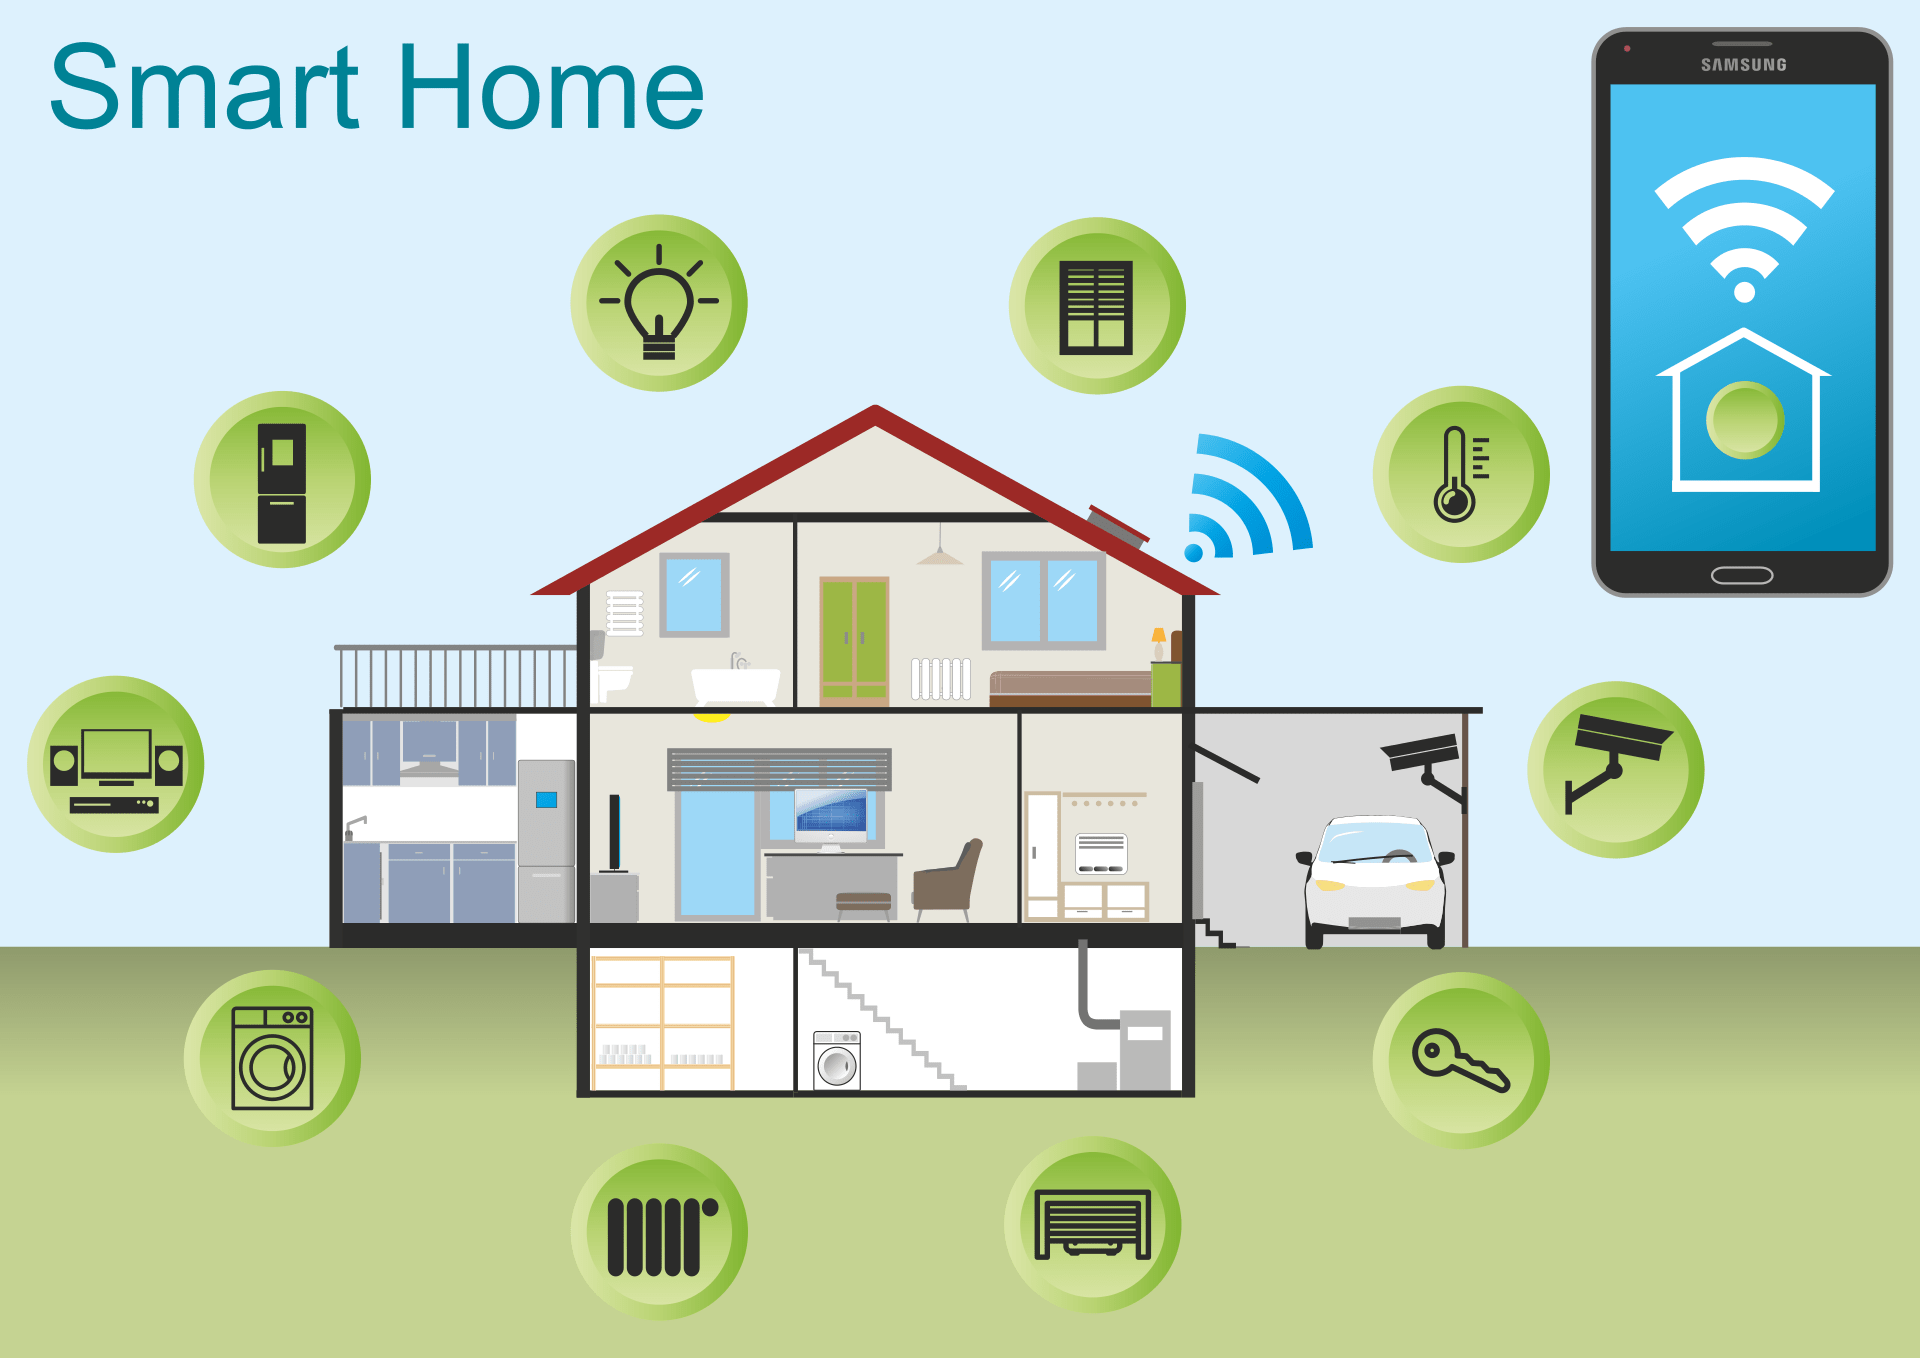
\includegraphics[width=\textwidth]{shome.png}
        \label{fig:my_label}
    \end{figure}
\end{frame}
\end{document}